\documentclass[conference]{IEEEtran}
\usepackage{graphicx}
\usepackage{cite}
\usepackage{amsmath}
\usepackage{hyperref}
\usepackage{tikz}
\usetikzlibrary{shapes.geometric, arrows, positioning}

\title{Graph Data Processing and Distributed Streaming Pipelines: A Portfolio Report}
\author{
    \IEEEauthorblockN{Abhisekhar Bharadwaj Gandavarapu}
    \IEEEauthorblockA{School of Computing and Augmented Intelligence\\
    Arizona State University\\
    Tempe, Arizona, USA\\
    Email: agandav1@asu.edu}
}

\begin{document}

\maketitle

\begin{abstract}
This portfolio report presents the design, implementation, and integration of two complementary data processing systems developed as part of CSE 511: Data Processing at Scale. The first project focuses on graph data processing using containerized Neo4j deployments with classical graph algorithms, while the second project extends this foundation to a distributed streaming architecture using Apache Kafka and Kubernetes orchestration. Together, these projects demonstrate the practical application of modern data engineering principles for processing urban transportation data at scale. The work highlights the synergy between graph databases, container technologies, and distributed messaging systems in building robust data pipelines.
\end{abstract}

\section{Introduction}

The proliferation of urban mobility data has created unprecedented opportunities for understanding transportation patterns and optimizing city infrastructure. Modern cities generate vast quantities of trip records from taxicabs, ride-sharing services, and public transit systems. Processing this data effectively requires sophisticated tools that can capture the inherent relationships between locations while handling continuous data streams in real-time.

This portfolio presents two interconnected projects that address these challenges through complementary approaches. The first project establishes a foundation in graph data processing by modeling transportation networks as graphs, where geographic locations serve as nodes and individual trips form relationships between them. This graph representation enables the application of powerful algorithms such as PageRank and Breadth-First Search to derive insights about location importance and connectivity.

The second project extends this foundation into the distributed computing domain by constructing a real-time streaming pipeline. This pipeline ingests trip data through Apache Kafka message queues, processes records in a distributed Kubernetes environment, and persists the results to a Neo4j graph database. The integration of these technologies demonstrates how batch and streaming paradigms can coexist within a unified data architecture.

The NYC Yellow Taxi dataset from March 2022 serves as the common data source across both projects, providing realistic trip records with pickup and dropoff locations, distances, fares, and timestamps \cite{nyctlc2022}. By focusing on trips within the Bronx borough, the projects work with a meaningful subset of data that exhibits the connectivity patterns and traffic flows characteristic of urban transportation networks.

\section{Explanation of the Solution}

\subsection{Project 1: Containerized Graph Data Processing}

The first project establishes an automated, reproducible environment for graph database operations through containerization. The system architecture consists of three primary layers: the container infrastructure, the graph database engine, and the algorithmic processing layer.

\subsubsection{Container Infrastructure}

The deployment leverages Docker to create a self-contained environment that encapsulates all dependencies required for Neo4j operation \cite{docker2023}. The container image builds upon Ubuntu 22.04 as a base operating system, onto which Java runtime, Python libraries, and the Neo4j database server are installed. This approach ensures consistent behavior across different host environments, eliminating the traditional challenges of dependency management and environment configuration.

The container configuration exposes two network ports: port 7474 for the Neo4j Browser web interface and port 7687 for the Bolt protocol used by application clients. This networking setup allows external applications to query the database while the database engine itself remains isolated within the container.

\subsubsection{Graph Data Model}

The data model transforms tabular trip records into a property graph structure suitable for Neo4j storage. Each unique pickup or dropoff location identifier becomes a Location node, with the location ID stored as a property. Trips between locations manifest as directed TRIP relationships connecting origin nodes to destination nodes.

This transformation preserves essential trip attributes as relationship properties, including the travel distance, fare amount, and temporal information for both pickup and dropoff events. The directed nature of relationships captures the asymmetric flow of traffic between locations, enabling analysis of one-way travel patterns that would be obscured in an undirected representation.

\subsubsection{Graph Algorithms}

The analytical layer implements two classical graph algorithms using the Neo4j Graph Data Science library \cite{neo4jgds2023}. PageRank evaluates the relative importance of each location within the transportation network by considering both the number of incoming trips and the importance of origin locations. Locations that receive trips from many other high-traffic locations receive correspondingly higher PageRank scores, revealing central hubs within the network.

Breadth-First Search provides pathfinding capabilities to determine the shortest route between any pair of locations. The algorithm explores the graph level by level, guaranteeing discovery of minimum-hop paths between origins and destinations. This capability supports route planning applications and network connectivity analysis.

\subsection{Project 2: Distributed Streaming Pipeline}

The second project constructs a distributed data pipeline that processes trip records in real-time, demonstrating the integration of multiple distributed systems technologies within a Kubernetes-orchestrated environment.

\subsubsection{Orchestration Layer}

Kubernetes serves as the orchestration platform, managing the deployment, scaling, and networking of all pipeline components \cite{kubernetes2023}. The system deploys multiple services including Zookeeper for distributed coordination, Kafka for message streaming, Neo4j for graph storage, and a custom connector service for data transformation.

Each component runs as a Kubernetes Deployment with associated Services that provide stable network endpoints. This architecture enables components to discover and communicate with each other through DNS-based service names, abstracting away the complexity of individual pod IP addresses.

\subsubsection{Message Streaming Layer}

Apache Kafka provides the messaging backbone that decouples data producers from consumers \cite{kafka2023}. The Kafka deployment runs within the Kubernetes cluster, coordinated by Zookeeper for cluster membership and configuration management. Kafka's topic-based publish-subscribe model allows the data producer to stream trip records without knowledge of downstream consumers.

The data producer application reads trip records from the source dataset, applies filtering criteria to select Bronx-area trips, transforms records to JSON format, and publishes each record to a designated Kafka topic. This streaming approach simulates real-time data arrival, with configurable delays between records to control ingestion rate.

\subsubsection{Connector Layer}

A Kafka Connect-based connector bridges the streaming and storage layers by consuming records from Kafka topics and persisting them to Neo4j. The connector interprets incoming JSON records, extracts location identifiers and trip attributes, and executes Cypher queries to create corresponding nodes and relationships in the graph database.

This connector architecture follows the Extract-Transform-Load pattern common in data engineering, where extraction occurs from Kafka, transformation handles format conversion and data validation, and loading creates graph structures in Neo4j. The connector runs as a separate Kubernetes deployment, scaling independently from other pipeline components.

\begin{figure}[t]
\centering
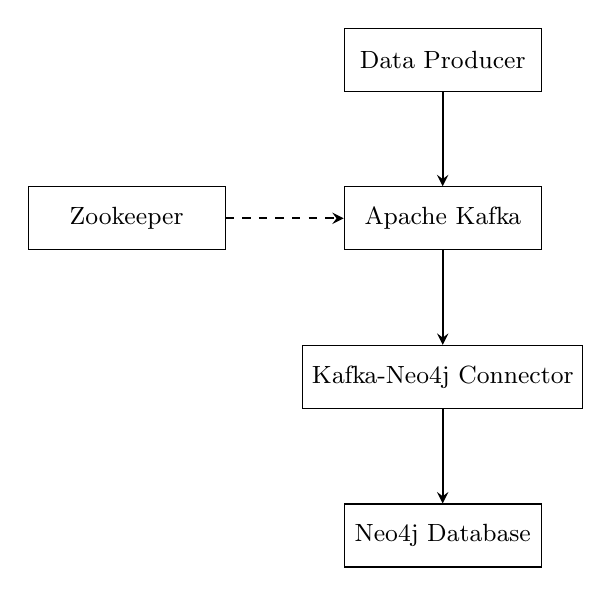
\begin{tikzpicture}[
    node distance=1.2cm,
    box/.style={rectangle, draw, minimum width=2.5cm, minimum height=0.8cm, text centered, font=\small},
    arrow/.style={->, >=stealth, thick}
]
    \node[box] (producer) {Data Producer};
    \node[box, below=of producer] (kafka) {Apache Kafka};
    \node[box, below=of kafka] (connector) {Kafka-Neo4j Connector};
    \node[box, below=of connector] (neo4j) {Neo4j Database};
    \node[box, left=1.5cm of kafka] (zk) {Zookeeper};
    
    \draw[arrow] (producer) -- (kafka);
    \draw[arrow] (kafka) -- (connector);
    \draw[arrow] (connector) -- (neo4j);
    \draw[arrow, dashed] (zk) -- (kafka);
\end{tikzpicture}
\caption{Architecture of the distributed streaming pipeline showing data flow from producer through Kafka messaging to Neo4j storage, with Zookeeper providing coordination services.}
\label{fig:pipeline}
\end{figure}

\subsubsection{Integration with Project 1}

The distributed pipeline produces graph structures compatible with those created in Project 1. The same Location nodes and TRIP relationships emerge from the streaming process, enabling the same PageRank and Breadth-First Search algorithms to operate on dynamically ingested data. This compatibility demonstrates how batch and streaming architectures can converge on a common data model.

\section{Description of the Results}

Both projects were successfully implemented and validated through automated testing procedures that verified correct behavior at each layer of the system.

\subsection{Project 1 Results}

The Docker image built successfully without requiring manual intervention during the build process. Upon container startup, the Neo4j database service initialized correctly and became accessible through both the web browser interface and the Bolt protocol.

Data loading completed successfully, creating Location nodes for each unique pickup and dropoff location identifier within the Bronx area. The TRIP relationships captured trip attributes accurately, with distance and fare values preserved as floating-point properties and timestamps stored in Neo4j's native datetime format.

The PageRank algorithm execution identified the most and least significant locations within the transportation network. High-ranking locations corresponded to areas with substantial incoming trip volume from diverse origins, while low-ranking locations represented peripheral areas with limited connectivity. The algorithm converged within the specified iteration limit, producing stable scores across multiple executions.

Breadth-First Search correctly identified shortest paths between specified location pairs. The algorithm handled cases where paths existed between distant locations, returning the complete sequence of intermediate nodes. For disconnected location pairs, the algorithm appropriately returned empty results rather than failing.

\subsection{Project 2 Results}

Kubernetes successfully orchestrated the deployment of all pipeline components. Zookeeper achieved a running state first, enabling Kafka to establish cluster coordination. The Neo4j Helm chart deployment created the graph database pod with the GDS plugin enabled for graph algorithm support.

The Kafka topic for trip data was automatically created when the first record was produced, demonstrating Kafka's auto-topic creation capability. Message production proceeded smoothly, with the producer logging confirmation for each successfully published record.

The Kafka-Neo4j connector established connections to both Kafka and Neo4j services, beginning consumption of trip records from the designated topic. Records flowed through the pipeline with observable latency of approximately 250 milliseconds per record, matching the configured production interval.

Query validation against the Neo4j database confirmed successful graph creation. Location nodes appeared as records were consumed, with TRIP relationships accumulating between them. The graph structure matched expectations from the source data, with the same filtering criteria applied during production reflected in the stored records.

Port forwarding enabled external access to both Neo4j and Kafka services from outside the Kubernetes cluster, supporting both the data producer application and the automated test suite. The complete pipeline demonstrated end-to-end functionality from data source through message streaming to graph storage.

\section{Contributions}

This portfolio represents individual work completed as a solo project for CSE 511. All implementation, testing, and documentation were performed independently, though conceptual discussions with course instructors and teaching assistants helped clarify requirements and resolve technical questions.

My personal involvement encompassed the complete development lifecycle across both projects. For Project 1, I designed the Dockerfile structure to satisfy the specified requirements, implemented the data loading logic to transform parquet files into graph structures, and developed the algorithm implementations using the GDS library interface.

For Project 2, I created the Kubernetes manifest files for each service deployment, configured the Helm values for Neo4j installation, developed the data producer application for Kafka message streaming, and integrated the connector component to bridge Kafka with Neo4j.

Throughout both projects, I iteratively debugged configuration issues, refined data transformation logic based on test feedback, and validated outputs against expected results. The learning process involved substantial independent research into Neo4j capabilities, Docker best practices, Kubernetes networking concepts, and Kafka architecture.

\section{Skills, Techniques, and Knowledge Gained}

These projects provided substantial learning opportunities across multiple technology domains, reinforcing theoretical concepts from course materials through practical implementation experience.

\subsection{Containerization and Reproducibility}

Working with Docker deepened my understanding of how containerization supports reproducible computing environments. The discipline of specifying all dependencies explicitly in a Dockerfile revealed the implicit assumptions that traditional development environments often hide. I gained practical experience with multi-stage builds, layer caching, and the trade-offs between image size and build complexity.

\subsection{Graph Database Concepts}

Neo4j introduced me to the property graph model and the Cypher query language. Unlike relational databases where relationships emerge from join operations, graph databases treat relationships as first-class entities that can carry properties and be traversed efficiently. The GDS library demonstrated how graph algorithms that would require complex implementations in traditional databases become straightforward library calls when working with native graph storage.

\subsection{Distributed Systems Fundamentals}

The Kubernetes deployment exposed fundamental distributed systems concepts including service discovery, container orchestration, and declarative configuration management. I learned how Kubernetes abstracts infrastructure concerns, allowing developers to specify desired states while the platform handles actual deployment and recovery.

\subsection{Stream Processing Patterns}

Apache Kafka introduced publish-subscribe messaging patterns and the concept of durable message logs. Unlike traditional message queues where consumption removes messages, Kafka's log-based architecture enables multiple consumers to process the same data at different paces. The Kafka Connect framework demonstrated how streaming platforms integrate with external systems through standardized connector interfaces.

\subsection{System Integration}

Perhaps the most valuable learning came from integrating multiple technologies into cohesive systems. Each component required understanding not just in isolation but in relation to others: how Docker exposes ports for Neo4j connectivity, how Kubernetes services enable inter-pod communication, how Kafka brokers coordinate with Zookeeper, and how connectors bridge streaming and storage systems. This integration experience developed a systems-level perspective that individual technology tutorials cannot provide.

\section{Conclusion}

This portfolio demonstrates the practical application of modern data engineering technologies to urban transportation data processing. Through containerized graph databases and distributed streaming pipelines, the projects illustrate how complementary technologies combine to address different aspects of large-scale data processing. The skills and knowledge gained through this work provide a foundation for continued exploration of data-intensive systems and distributed computing architectures.

\begin{thebibliography}{00}

\bibitem{nyctlc2022}
NYC Taxi and Limousine Commission, ``TLC Trip Record Data,'' NYC Open Data, 2022. [Online]. Available: https://www.nyc.gov/site/tlc/about/tlc-trip-record-data.page

\bibitem{docker2023}
Docker Inc., ``Docker Documentation,'' 2023. [Online]. Available: https://docs.docker.com/

\bibitem{neo4jgds2023}
Neo4j Inc., ``Neo4j Graph Data Science Library Manual,'' 2023. [Online]. Available: https://neo4j.com/docs/graph-data-science/current/

\bibitem{kubernetes2023}
The Linux Foundation, ``Kubernetes Documentation,'' 2023. [Online]. Available: https://kubernetes.io/docs/

\bibitem{kafka2023}
Apache Software Foundation, ``Apache Kafka Documentation,'' 2023. [Online]. Available: https://kafka.apache.org/documentation/

\end{thebibliography}

\end{document}


